\newpage

\section{Задание 2.}

Область в $\mathbb{R}^2$ ограничена данными кривыми. Найти площадь с помощью двойного интеграла, выполнить рисунок.

$$ y^2 - 2y+ x^2 = 0, y^2 - 6y+x^2 = 0, y = \dfrac{x}{\sqrt{3}}, x = 0$$

Преобразуем данные равенства, чтобы было легче изобразить.

$$ \left(y^2 - 2y +1\right) - 1  + x^2 = 0, \left(y^2 - 2\cdot 3\cdot y + 3^2\right) -3^2 +x^2 = 0, y = \dfrac{x}{\sqrt{3}}, x = 0$$

$$ \left(y - 1\right)^2 + x^2 = 1^2, \left(y^2 - 3\right)^2 +x^2 = 3^2, y = \dfrac{x}{\sqrt{3}}, x = 0$$

Итого мы имеем два круга, один с радиусом $1$ и центром в $(0,1)$, и второй с радиусом $3$ и центром в $(0,3)$ и прямую с наклоном $\dfrac{1}{\sqrt{3}}$.

\begin{figure}[h!t]
    \centering
    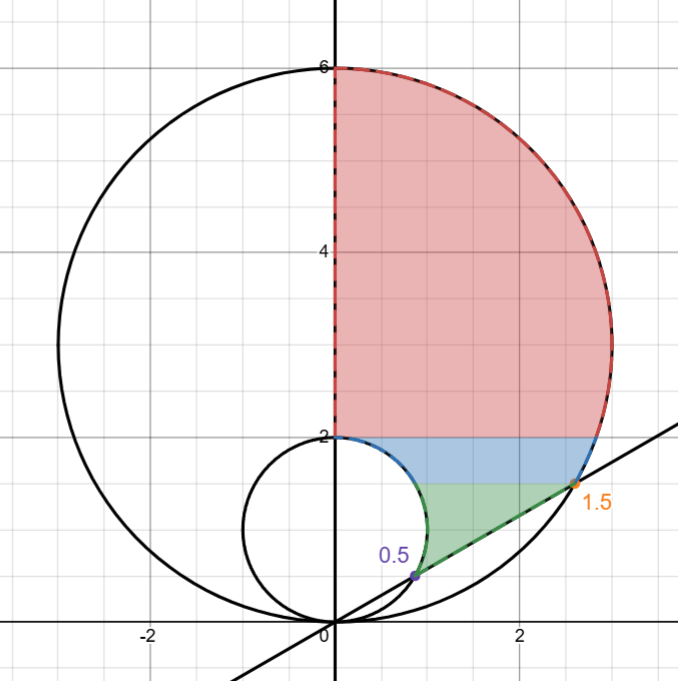
\includegraphics[width=0.3\linewidth]{Task2/Figure_shape.png}
    \caption{Задание 2. Области интегрирования \underline{\href{https://www.desmos.com/Calculator/spyqn3wlhu}{(Desmos)}}. }
\end{figure}

Нужный нам интеграл можно записать в следующем виде.

$$\iint\limits_{\text{Фигура}}1\,dx\, dy = \iint\limits_{\text{Красная}}1\,dx\, dy + \iint\limits_{\text{Синяя}}1\,dx\, dy + \iint\limits_{\text{Зеленая}}1\,dx\, dy = $$
$$= \int_2^6 \,dy \int_{0}^{\sqrt{9-\left(y-3\right)^{2}}}\,dx + \int_{1.5}^{2} \,dy \int_{\sqrt{1-\left(y-1\right)^{2}}}^{\sqrt{9-\left(y-3\right)^{2}}}\,dx + \int_{0.5}^{1.5}\int_{\sqrt{1-\left(y-1\right)^{2}}}^{y\sqrt{3}}\,dx = $$
$$=\int_2^6 \sqrt{9-\left(y-3\right)^{2}}\,dy + \int_{1.5}^{2} \sqrt{9-\left(y-3\right)^{2}} - \sqrt{1-\left(y-1\right)^{2}}\, dy + \int_{0.5}^{1.5} y\sqrt{3} - \sqrt{1-\left(y-1\right)^{2}}\, dy = $$
$$=\int_2^6 \sqrt{9-\left(y-3\right)^{2}}\,dy + \int_{1.5}^{2} \sqrt{9-\left(y-3\right)^{2}}\,dy - \int_{1.5}^{2}\sqrt{1-\left(y-1\right)^{2}}\, dy + \int_{0.5}^{1.5} y\sqrt{3}\,dy - \int_{0.5}^{1.5}\sqrt{1-\left(y-1\right)^{2}}\, dy =$$
$$=\int_{1.5}^6 \sqrt{9-\left(y-3\right)^{2}}\,dy - \int_{0.5}^{2}\sqrt{1-\left(y-1\right)^{2}}\, dy - \int_{0.5}^{1.5}y\sqrt{3}\,dy  = $$
$$=\int_{-1.5}^3 \sqrt{9-t^{2}}\,dt - \int_{-0.5}^{1}\sqrt{1-t^{2}}\, dt - \sqrt{3}\int_{0.5}^{1.5}y\,dy  $$

Воспользуемся тем фактом, что знаем, как выглядит первообразная для одной из функций.

$$\int \sqrt{a^2 - x^2} dx = \frac{a^2}{2} \arcsin\left(\frac{x}{a}\right) + \frac{x}{2} \sqrt{a^2 - x^2} + C$$

Тогда, возвращаясь к нашему интегралу

$$= \left[ \frac{9}{2} \arcsin \left( \frac{t}{3} \right) + \frac{1}{2} t \sqrt{9 - t^2} \right]_{-1.5}^{3} - \left[ \frac{1}{2} \arcsin(t) + \frac{1}{2} t \sqrt{1 - t^2} \right]^{1^{-0.5}} + \sqrt{3} \left[ \frac{y^2}{2} \right]^{1.5}_{0.5} = $$

$$=\frac{9\pi}{4} - \left(-\frac{3\pi}{4} - \frac{9\sqrt{3}}{8}\right) - \left(\frac{\pi}{4} - \left( -\frac{\pi}{12} - \frac{\sqrt{3}}{8} \right) \right) +\sqrt{3} =$$

$$3=\pi + \frac{9\sqrt{3}}{8} - \left(\frac{\pi}{3} + \frac{\sqrt{3}}{8}\right) - \sqrt{3} = \boxed{\frac{8\pi}{3}}$$
